\section{Project Management}\label{Project Management} 
    In this section, we'll take look at how we organized the team, a brief risk assessment, and an evaluation of the work process. 
    
    \subsection{Team Organization}\label{Team Organization} 
        This section describes in detail how we organize ourselves and how we split roles and tasks among the team members. We have a flat team structure\footnote{Flat organization structure is a structure with few or no levels of intervening management. The idea is that well-trained workers will be more productive when they are directly involved with decision making. [\url{http://en.wikipedia.org/wiki/Flat_organization}]}  and have shifted our focus accordingly over to team communication. 
    
    \subsubsection{Team Structure}\label{Team Structure}
    We already know each other coming into the project so we have chosen a flat organizational structure (Fig:\ref{fig:TeamOrganizationchart}), with no intervening levels of management, since all decisions within the team will more or less be made by all the members together either way. Relying on the entire group for decisions will both involve and invest everyone in the project and will work well with our already existing group dynamic.

    \begin{figure}[H]
        \centering
        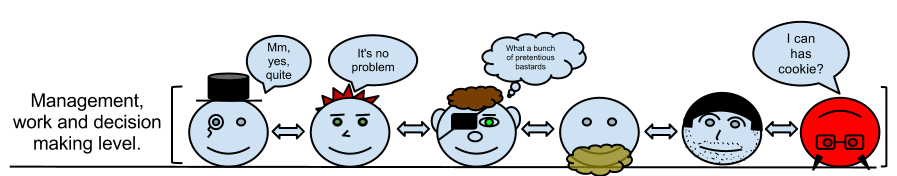
\includegraphics[width=\textwidth]{TeamOrganizationchart}
        \caption{Team Organization chart}
        It was made during lunch, but the general principle still remains, that the structure is flat.
        \label{fig:TeamOrganizationchart}
    \end{figure}
    
    %Why changing roles does not work in our structure and how we solve the challenges that might occur in this association. 
    As the structure shows in the chart (Fig:\ref{fig:TeamOrganizationchart}), there is no difference in what responsibility level anyone have, or what role one has. The concept of changing roles weekly is good for a learning situation, but very inefficient where knowledge and research are key components in a limited timed project. We anticipate that the time for this project probably won't be sufficient for any role changes, and therefore we have to keep people focused on the task they have been assigned. The efficiency of the current task relies on having the current research fresh in mind. If we were to change the roles every week, the newly assigned person would spend a lot of time getting up to date at the beginning of every week, which in turn wouldn't yield any measurable gains. 
    
    Rather than focus on responsibilities within the group, we've chosen to focus on tasks.
The task will to some degree still represent areas of responsibilities, and since tasks will be spread across several group members, we don't run the risk of  a single missing member crippling the entire group. Instead the remaining member$($assigned$)$ to a task will be able to pick of the slack. This, together with thorough documentation of a members knowledge, will just about eliminate the problems associated with an absent group member.
        
    Further, the team structure and the distribution of responsibility gives us the chance to define how we want to deal with task and their priority. The work flow that we have makes us prioritize tasks continuously and get the most pressing task done at the correct time. It's similar to a max heap. We put tasks in to the heap, heapify(prioritise tasks) and choose(pop) the maximized task, the task that has the highest priority. 
    
    %Task division and delegation.
    When we choose a task we consider the person's interest, experience and existing knowledge. Most times the tasks fall naturally to one person that has worked with similar tasks earlier in the project. Other times there is more of lottery, where the task has no prerequisites. Often we rely on a person's initiative to take a task or we easily delegate them with a question, "Can someone do that?". Task delegation and sharing the work load has not been a problem so far in the project.
    
    %benefits of a flat team structure. 
    
    \subsubsection{Team communication}\label{Team communication}
    We decided that we will work together from 10 to 16, Monday through Thursday every week, with allowed exceptions for lectures and such. Group members can also work in their free time to make up for missed collaboration hours or to just put in some extra work. This means more work than the course requires, but we decided that we want to do it this way so we can either take some time off now and then, or have more time for the exams in May.

    We will not be able to have frequent face to face meetings with the customer, because the customer is located in Oslo. We decided to have weekly meetings using Skype instead, as well as e-mail communication as needed. Since we have seen what happens in projects where there is little to no communication, we decided, in agreement with the costumer, that we at least wanted to have weekly meetings in order to keep a good dialog with the customer, and also give them the opportunity to take part in the development of the project. 
    
    \subsubsection{Roles}\label{roles}
    
    Our team structure is discussed in \textit{Team Structure} (ref:\ref{Team Structure}). It describes the general structure and the ideal situation and delegation. 
    
    But to make this work in practice roles are unconsciously delegated to different people. A person ends up with a role loosely based on the first delegation of a task. 
    
    When a person works on a task, experience is gained. This experience is useful when the same, or a similar, task occurs again. 
    
    This means that the person best suited to deal with this task is the same person that dealt with it last time. To get the most efficient result the same person is picked to deal with this task as well. 

    A good thing about this is the that the same person don't have to waste time to read up on necessary information to deal with the task at hand.  
    
    How the roles actually worked is described in section \ref{evaluation:team organization}.
        
    \subsection{Risk Assessment}\label{Risk Assessment}
     To help us avoid most problems we created a risk list which should contain most of the problems that we can encounter during this project. A risk list can never cover all the cases that could occur, but we think that our risk list contains most of them. To cover the last cases which we might have overlooked we decided that we would add some \textit{Risk Management} strategies to this section to explain how we will handle unforeseen risk as they appear. 
     
     To handle most of the risks that we have not written down in our risk list we will try to have a close dialog with the customer so that if an unforeseen risk should occur they will be informed about it. That way we can discus the problem together and come up with a solution that is satisfactory for everyone. Having this open dialog with the customer also ensures that they won't be surprised by any choices we make.
     
    A natural approach to risk management will be to first accept the situation and involve the whole group. Then we will assess the situation and pin point the problem and it's cause. When the problem and it's cause is found there will be a lot of different approaches to solve the situation, depending a lot on the actual situation. 
    
    When a risk is present and confirmed we have to deal with it as best we can. The way we would do this is to open, frank and honest. This will put all the information on the table and we can then continue the process with a better understanding of the situation. Then we would continue with finding a solution and coordinate our collaboration within the group and with the customer and supervisor to ensure the best solution possible.

    \subsection{Progress tracking and Documentation}\label{Progress tracking and Documentation}
    In the beginning we had a summary every day where we wrote what we were working on and what had to be done. We stopped doing this after we got good activity plans because the daily summaries became unnecessary. 
    
    \begin{figure}[H]
        \centering
        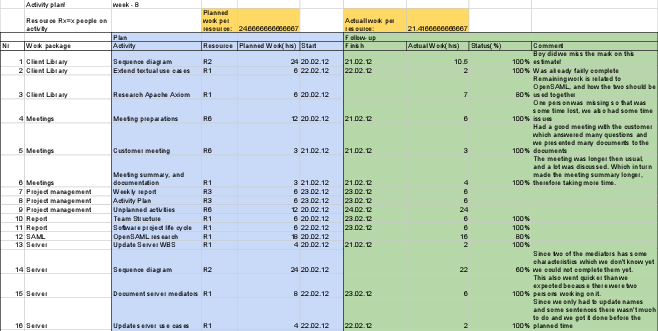
\includegraphics[width=\textwidth]{Week8activityplan}
        \caption{Example Activity plan}
        This figure displays the structure of our activity plans. It's meant as an overview. See the appendix for full weekly reports. 
        (ref:\ref{Attachments:Activity Plans})
        \label{fig:Week8activityplan}
    \end{figure}
    
    The activity plans(Fig:\ref{fig:Week8activityplan}) now have the role of our day to day summaries and work progress. We update the activity plan as we go along. This way we have a complete overview of tasks and work hours that are planned this week. As we update the activity plan we have an overview of the work done this week and where we have missed with our time estimation. 
    
    \begin{figure}[H]
        \centering
        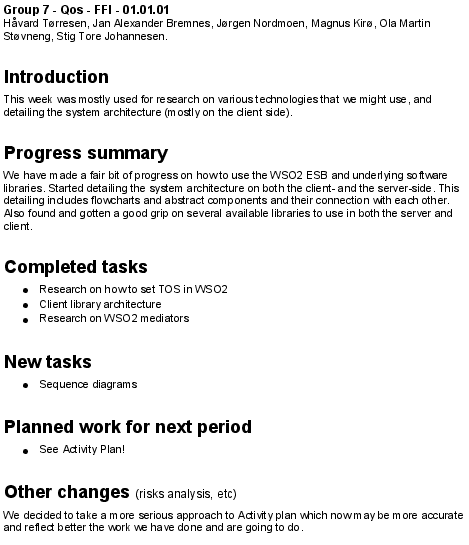
\includegraphics[scale=0.5]{Week7statusreport}
        \caption{Status report example}
        This is an example of one of our status reports. We create them every week. All the weekly reports can be found in appendix \ref{Attachments:Weekly Reports}
        \label{fig:Week7statusreport}
    \end{figure}
    
    As we can see in the weekly report (Fig:\ref{fig:Week7statusreport}) the status report has a standard setup. We created a template early in the project so that we could reuse it later and reduce work. In the process of creating the template we put some thought into it so that we would get a template that would work throughout the project without further changes. Despite the thought process of creating the templates, we had to make some small changes throughout the project.
    
       \subsection{Progress Evaluation}\label{Progress Evaluation}
    We have assessed our progress every week. This has been done with weekly reports, schedules and activity plans. These can be seen in the attachments appendix (ref:\ref{Attachments}).
    
    This documentation process has taken up a substantial amount of time every Thursday. The documentation part that we have done every week consists mainly of three things. Writing the weekly report, updating the activity plan and creating the next activity plan. 
    
    The time this has taken varies quite a bit. This is because some weeks we have nothing more then "Everything went according to plan." to write in the weekly report and the activity plans quite often plans themselves to some extent. Meaning the taskst that has to be done is dictated by the taske that has been done, and the activity plan only has to be filled out.
    
    The weekly reports and activity plans have been used to inform the customer and supervisor of our progress and get feedback on our progress. If the progress wasn't good enough we would get feedback on that. 
    
    The schedules tracked our time usage and is kind of a log for what has been done by whom. We do not use the schedules to point out people that has put down more or less work in this project. It is merely a document for the group to keep track of things. 
    
    
